\documentclass[10pt,prd,aps,nofootinbib,superscriptaddress]{revtex4}
\usepackage{epsf,graphicx,xcolor,amsmath}

\newcommand{\beq}{\begin{equation}}
\newcommand{\eeq}{\end{equation}}
\newcommand{\bea}{\begin{eqnarray}}
\newcommand{\eea}{\end{eqnarray}}
\newcommand{\nn}{\nonumber}



\begin{document}

\title{$\Upsilon$ photoproduction on the proton at an Electron-Ion Collider}
\author{Oleksii Gryniuk}
\affiliation{Institut f\"ur Kernphysik \& PRISMA$^+$  Cluster of Excellence, Johannes Gutenberg Universit\"at,  D-55099 Mainz, Germany}
\author{Sylvester Joosten}
\affiliation{ANL...}
\author{Zein-Eddine Meziani}
\affiliation{ANL...}
\author{Marc Vanderhaeghen}
\affiliation{Institut f\"ur Kernphysik \& PRISMA$^+$  Cluster of Excellence, Johannes Gutenberg Universit\"at,  D-55099 Mainz, Germany}
\noaffiliation
\date{\today}

\begin{abstract}
abstract...
\end{abstract}

\maketitle

\tableofcontents


\section{Introduction}

\newpage

\section{$\Upsilon$ proton forward scattering amplitude}

We consider the spin-averaged $\Upsilon p \to \Upsilon p$ forward elastic scattering process, which is described by an invariant amplitude $T_{\Upsilon p}$, depending on the crossing variable $\nu$. The latter is defined in terms of the Mandelstam invariant $s$ as:
\bea
\nu = \frac{1}{2} (s - M^2 - M_\Upsilon^2),
\eea
where $M (M_\Upsilon)$ stand for the masses of the proton $(\Upsilon)$ respectively.  
The forward differential cross section for the $\Upsilon \, p \to \Upsilon \, p$ scattering process can then be expressed as:
\bea
\frac{d \sigma}{dt} \biggr|_{t = 0} (\Upsilon p \to \Upsilon p) = \frac{1}{64 \, \pi \, s \, q_{\Upsilon p}^2} \, \big| T_{\Upsilon p}(\nu) \big|^2,
\eea
where in the forward direction the momentum transfer $t = 0$, and where $q_{\Upsilon p}$ denotes the magnitude of the $\Upsilon$ three-momentum in the c.m. frame, given by:
 \bea 
 q_{\Upsilon p}^2  = \frac{1}{4 s} \left[ s - (M_\Upsilon + M)^2 \right] \left[ s - (M_\Upsilon - M)^2 \right].
 \eea 
 
The imaginary part of the amplitude $T_{\Upsilon p}$ can be obtained as sum of elastic and inelastic discontinuities:
\bea
\Im T_{\Upsilon p}(\nu)  = \theta(\nu - \nu_{el}) \,  {\rm Disc}_{\rm el} T_{\Upsilon p}(\nu) +   \theta(\nu - \nu_{inel}) \,  {\rm Disc}_{\rm inel} T_{\Upsilon p}(\nu).
\label{eq:disctot}
\eea
The elastic discontinuity starts from elastic threshold $s = s_{el} = (M_\Upsilon + M)^2 = 108.13$~GeV$^2$, or equivalently $\nu_{el} = M_\Upsilon M = 8.88$~GeV$^2$, whereas the inelastic discontinuity 
starts at the $B \bar B$ meson production threshold, corresponding with $s_{inel} = (M + 2 M_B)^2 = 132.18$~GeV$^2$, or equivalently $\nu_{inel} = 20.90$~GeV$^2$. 

Analogous to the $J/\psi$ case~\cite{Gryniuk:2016mpk}, 
we will parameterize the elastic and inelastic discontinuities of the $\Upsilon p$  forward scattering amplitude 
by the following 3-parameter forms, for $x = {\rm el/inel}$:
\bea
{\rm Disc}_{x} T_{\Upsilon p}(\nu)  &=& 
C_{x} \left( 1 - \frac{\nu_{x}}{\nu} \right)^{b_{x}}  \left( \frac{\nu}{\nu_{x}} \right)^{a_{x}} ,
\label{eq:discx} 
\eea
where the factors $\sim (1 - \nu_x / \nu)^{b_x}$  
determine the behavior around the respective threshold $\nu_x$, and the 
factors  $\sim \nu^{a_x}$ determine the Regge behavior of the amplitude at large $\nu$. 
In the following we will discuss how we can determine the respective parameters 
appearing in the elastic and inelastic discontinuities. 

We use the vector meson dominance (VMD) assumption to relate the $\Upsilon p$ elastic cross section 
$\sigma_{\Upsilon p}^{el}$ to the total $\gamma p \to \Upsilon p$ photoproduction cross section~\cite{Barger:1975ng,Redlich:2000cb}, which fixes the 
discontinuity across the elastic cut as: 
\bea
{\rm Disc}_{\rm el} T_{\Upsilon p}(\nu)  &=& 2 \sqrt{s} \, q_{\Upsilon p} \sigma_{\Upsilon p}^{el} 
=  2 \sqrt{s} \, q_{\Upsilon p}  \left( \frac{M_\Upsilon}{e f_\Upsilon} \right)^2 \left( \frac{q_{\gamma p}}{q_{\Upsilon p}} \right)^2 \, 
\sigma (\gamma p \to \Upsilon p), 
\label{eq:sigmael}
\eea
with electric charge $e$ given through $\alpha = e^2 / (4 \pi) \simeq 1/137$, and  where $f_\Upsilon$ is the $\Upsilon$ decay constant, which is obtained from the $\Upsilon \to e^+ e^-$ decay as 
\begin{eqnarray}
\Gamma_{\Upsilon \to ee} = \frac{4 \pi \alpha^2}{3} \frac{f_\Upsilon^2}{M_\Upsilon}.
\end{eqnarray}
The experimental value $\Gamma_{\Upsilon \to ee} =  1.34$~keV yields $f_\Upsilon = 0.238$~GeV. Furthermore, $q_{\gamma p}$ denotes the magnitude of the 
$\gamma$ three-momentum in the c.m. frame of the $\gamma p \to \Upsilon p$ process:
\bea
q_{\gamma p} = \frac{(s - M^2)}{2 \sqrt{s}}.
\eea

The discontinuity across the inelastic cut, ${\rm Disc}_{inel} T_{\Upsilon p}$, 
is related through the optical theorem to the $\Upsilon \, p \to b \bar b X$ inelastic cross section 
$\sigma_{\Upsilon p}^{inel}$, which is again related, using VMD, to the corresponding $\gamma p \to b \bar b X$ photoproduction cross section:
\bea
{\rm Disc}_{\rm inel} T_{\Upsilon p}(\nu) = 2 \sqrt{s} \, q_{\Upsilon p} \, \sigma_{\Upsilon p}^{inel}    
 = 2 \sqrt{s} \, q_{\Upsilon p} \,  \left( \frac{M_\Upsilon}{e f_\Upsilon} \right)^2  \left( \frac{q_{\gamma p}}{q_{\Upsilon p}} \right)^2 \,  \sigma (\gamma p \to b \bar b X). 
\label{eq:sigmainel}
\eea

Having fixed the imaginary part of $T_{\Upsilon p}$,  
the real part of $T_{\Upsilon p}$ is related to its imaginary part
through a once-subtracted forward dispersion relation:
\beq
\Re T_{\Upsilon p}(\nu) = T_{\Upsilon p}(0) + \frac{2}{\pi} \nu^2 \int_{\nu_{el}}^\infty d
\nu^\prime \frac{1}{\nu^\prime} \frac{\Im T_{\Upsilon p}(\nu^\prime)}{\nu^{\prime \, 2} - \nu^2},
\label{eq:disp}
\eeq
with $T_{\Upsilon p}(0) $ the subtraction constant at $\nu = 0$. In this work, the subtraction constant will be obtained by performing a fit of the 
differential $\gamma p \to \Upsilon p$  photoproduction cross section data at $t=0$, which is related to $T_{\Upsilon p}$ as:
\beq
\frac{d \sigma}{dt} \biggr|_{t = 0} (\gamma p \to \Upsilon p) 
= \left( \frac{e f_\Upsilon}{M_\Upsilon} \right)^2  \frac{1}{64 \, \pi \, s \, q_{\gamma p}^2} \, \big| T_{\Upsilon p}(\nu) \big|^2.
\label{eq:dsigmadt0_gapjpsip}
\eeq

The real part of the forward scattering amplitude at threshold $T_{\Upsilon p}(\nu_{el}) $ is directly related to the $\Upsilon p$ scattering length 
$a_{\Upsilon p}$ as:
\bea
T_{\Upsilon p}(\nu = \nu_{el}) = 8 \pi (M + M_\Upsilon) \, a_{\Upsilon p}. 
\eea
Analogously to the $J/\Psi$ case, 
we may relate a positive $\Upsilon p$ scattering length, corresponding to an attractive interaction, 
to an $\Upsilon$ binding energy $B_\Upsilon$ in nuclear matter, using a linear density approximation~\cite{Kaidalov:1992hd}:
\begin{eqnarray}
B_\Upsilon \simeq \frac{8 \pi (M + M_\Upsilon) a_{\Upsilon p}}{4 M M_\Upsilon} \, \rho_{nm},
\label{eq:nmbe}
\end{eqnarray}
where $\rho_{nm} \simeq 0.17$~fm$^{-3}$ denotes the nuclear matter density.



\section{Results and discussion}

In order to empirically determine the $\Upsilon p$ scattering length $a_{\Upsilon p}$, the strategy we use in this work follows our previous analysis for 
the $J/\psi p$ system~\cite{Gryniuk:2016mpk}. The data on the $\gamma p \to \Upsilon p$ and $\gamma p \to b \bar b X$ total cross sections 
are parameterized according to the three-parameter forms of Eq.~(\ref{eq:discx}) inserted into Eqs.~(\ref{eq:sigmael}) and (\ref{eq:sigmainel}).
This determines the total imaginary part in the dispersion integral of Eq.~(\ref{eq:disp}). The real part is then calculated from the dispersion integral  
and the subtraction constant is extracted from a fit to the differential $\gamma p \to \Upsilon p$ cross section extrapolated to $t = 0$, using Eq.~(\ref{eq:dsigmadt0_gapjpsip}).
 
At present, the exclusive $\Upsilon$ photoproduction database
consists of four datapoints from HERA~\cite{Adloff:2000vm, Breitweg:1998ki, Chekanov:2009zz}
(see Fig.~\ref{fig:sigmatot}, left panel). 
Furthermore at LHC energies, the $\gamma p \to \Upsilon p$ cross section has been extracted from central pp production data at LHCb~\cite{Aaij:2015kea} 
and from ultra-peripheral pPb collisions at  CMS~\cite{Sirunyan:2018sav}
For high energies $\sqrt{s} = W\sim100$ GeV, the differential cross section data shows an exponential t-dependence 
%corresponding to the dependence
\beq
\frac{d \sigma}{dt} (\gamma p \to \Upsilon p)
\;=\; A \cdot e^{Bt}, \quad \quad 
A = \frac{d \sigma}{dt} \biggr|_{t = 0} (\gamma p \to \Upsilon p) ,
\label{eq:bdef}
\eeq
with an empirical slope parameter $B(W = 100$~GeV$)=4.5\pm0.5$~GeV$^{-2}$~\cite{Chekanov:2009zz}. 
The exponential dependence of Eq.~(\ref{eq:bdef}) allows us to express the extrapolated value
 of the differential cross section at $t=0$ as
\beq
A  \simeq B e^{- B t_{\rm min}} \cdot\sigma (\gamma p \to \Upsilon p),
\label{eq:brel}
\eeq
where
\beq
t_\mathrm{min} = M_\Upsilon^2 - 2q_{\gamma p} \left(\sqrt{q_{\Upsilon p}^2 + M_\Upsilon^2} - q_{\Upsilon p}\right)
\eeq
is the minimum (modulo) physical momentum transfer, corresponding to the forward scattering ($\theta_{\gamma \Upsilon}=0$).

The inclusive $b \bar b$ photoproduction database is represented by one datapoint from HERA~\cite{Adloff:1999nr}.
Additionally, the lower energy cross section upper limit from EMC~\cite{Aubert:1981gx}
is added to guide the low-energy behaviour (see Fig.~\ref{fig:sigmatot}, right panel).

\begin{figure}
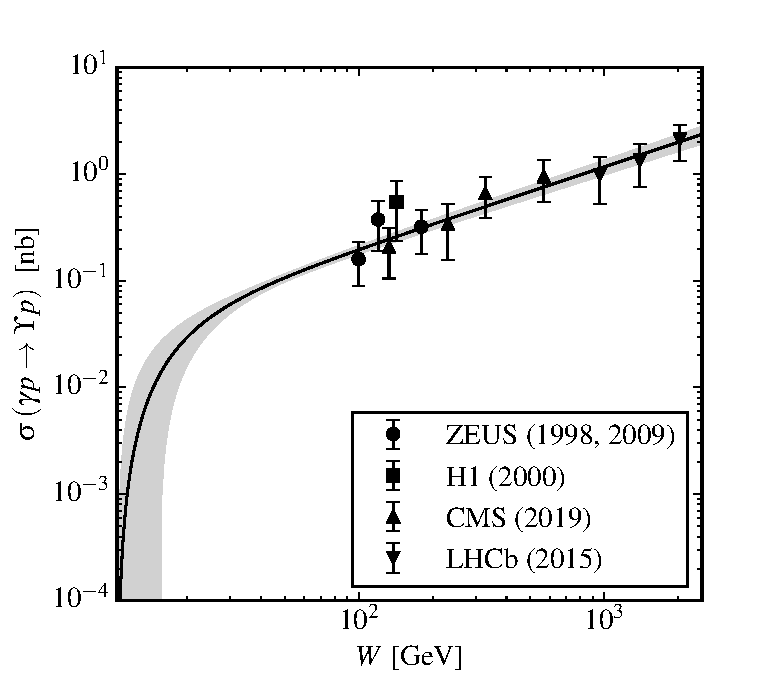
\includegraphics[width=0.49\textwidth]{si_y.pdf}
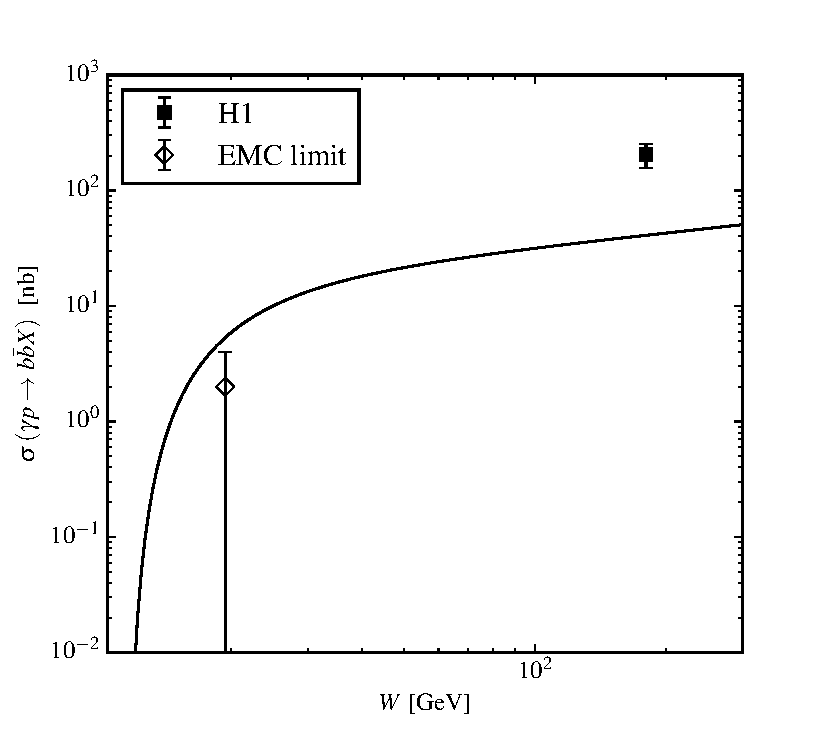
\includegraphics[width=0.49\textwidth]{si_bbX.pdf}
\caption{W-dependence of the $\gamma p \to \Upsilon p$ (left) and $\gamma p \to b \bar b X$ (right) total cross sections.
The curve is the result of our global fit with parameters given in Table~\ref{tab:fits}.
The elastic $\Upsilon$ photoproduction data are from HERA: H1~\cite{Adloff:2000vm}
and ZEUS~\cite{Breitweg:1998ki, Chekanov:2009zz}, and from LHC: LHCb~\cite{Aaij:2015kea} 
and CMS~\cite{Sirunyan:2018sav}. 
The simulated EIC datapoints shown are based on the differential in $t$ cross section points:
the fitted $Ae^{Bt}$ is integrated between $t_\mathrm{min}$ and $t_\mathrm{max}$.
The error bars of the EIC datapoints are propagated through the resulting covariance matrix of the $A$ and $B$ parameters.
The open beauty production data points are from HERA~\cite{Adloff:1999nr}, EMC~\cite{Aubert:1981gx}.}
\label{fig:sigmatot}
\end{figure}



The present database is insufficient to perform a high-quality fit using the forms of Eq.~(\ref{eq:discx}) with all the parameters unconstrained.
We may reasonably expect however, for a diffractive process, that the $a_x$ values are in general similar to those for the $J/\psi$.
The lack of low-energy data prevents a direct determination of the low-energy slope parameters $b_x$ of the cross sections at present.
We thus start by simply fixing all the low- and high-energy slope parameters to the $J/\psi$ values from~\cite{Gryniuk:2016mpk}:
\bea
a_{\rm el} = 1.38, &\quad& a_{\rm inel} = 1.20, \\
b_{\rm el} = 1.27, &\quad& b_{\rm inel} = 3.53 .
\eea
We then fit the elastic normalization constant $C_{\rm el}$ to the four datapoints of the elastic $\Upsilon$ photoproduction cross section, as shown in Fig.~\ref{fig:sigmatot} (left panel). 
In order to fit the inelastic normalization constant $C_{\rm inel}$, we make the observation from Fig.~\ref{fig:sigmatot} that around $W = 100$~GeV, the HERA data for the inelastic cross section are around 2 orders of magnitude larger than their elastic counterparts. We can thus safely assume that the amplitude $T_{\Upsilon p}$ entering the differential cross section in Eq.~(\ref{eq:dsigmadt0_gapjpsip}) is dominated by the imaginary part of the inelastic process, proportional to $C_{\rm inel}$. 
By then relating the cross section ratio of Eq.~(\ref{eq:brel}) to the slope parameter $B$ at $W=100$ GeV, 
we obtain the relation:
\beq
B (W = 100~{\rm GeV}) \simeq  
 \frac{C_{\rm inel}^2}{C_{\rm el}} \left[ \frac{1}{16 \pi W^2} \left( \frac{\nu}{\nu_{\rm inel}} \right)^{2 a_{\rm inel}} 
\left( \frac{\nu_{\rm el}}{\nu} \right)^{a_{\rm el}} \right]_{W = 100~{\rm GeV} } . 
\label{eq:Crel}
\eeq
Using the emprical slope parameter at $W = 100$~GeV and the fit value of $C_{\rm el}$, allows then to fix the normalization constant $C_{\rm inel}$. 
The final values of the total cross section parameters are listed in Table~\ref{tab:fits}. 
We obtain for the elastic photoproduction total cross section data $\chi^2/{\rm d.o.f.} = 0.3$ (11 points, 2 parameters).

\begin{table}[h]
\begin{tabular*}{\textwidth}{c @{\extracolsep{\fill}} cccc}
\hline
\hline
& \quad $x$ = el \quad & \quad $x$ = inel \quad\\
\hline
$C_x$ & $(14.60\pm3.69)\times 10^{-3}$ & $20.17\pm2.55$ \\
$b_x$ & $1.27$ & $3.53$ \\
$a_x$ & $1.38$ & $1.2$ \\
\hline
\hline
\end{tabular*}
\caption{Fit results for the coefficients entering the elastic discontinuity (second column, $x = el$), 
and the inelastic discontinuity (third column, $x = inel$).
The $b_x$ parameters are fixed from $J/\psi$ case result~\cite{Gryniuk:2016mpk}.
%\textcolor{red}{The errors are based on the covariance matrix.}
% The given uncertainties for the $a_{\rm el}$ and $C_{\rm el}$ parameters
% are the {\it uncorrelated} linear estimates based on the four data points of the elastic photoproduction.
% The uncertainty of $a_{\rm inel}$ is obtained similarly based on the two inelastic photoproduction points.
The $C_{\rm inel}$ parameter uncertainty is simply estimated as half of the relative uncertainty of $C_{\rm el}$
based on relation of Eq.~(\ref{eq:Crel}).
}
\label{tab:fits}
\end{table}


Having fixed the imaginary part of the amplitude $T_{\Upsilon p}$, we evaluate the dispersion integral of Eq.~(\ref{eq:disp}). 
The real part is then calculated from the dispersion relation up to the subtraction constant. 
Whereas at high energies (i.e. HERA energies) the differential cross section is largely dominated by its imaginary part, we get sizeable sensitivity to 
the real part at low to intermediate energies. We will explore in the following how to extract the subtraction constant from a fit to the 
 differential $\gamma p \to \Upsilon p$ cross section data at an Electron-Ion Collider at two energy settings, corresponding with the range 
 $W < 30$~GeV and $W < 50$~GeV.    

In order to perform a feasibility study of such forthcoming data, we will consider three scenarios for the subtraction constant in order to 
explore the data sensitivity to its extraction. 
The simplest scenario corresponds with having zero value of the subtraction constant. The real part of the $\Upsilon p$ scattering amplitude is then fully determined by its imaginary part through the dispersion integral. The resulting value of the $\Upsilon p$ scattering length is then extremely small, around $a_{\Upsilon p} \simeq 0.6 \times 10^{-3}$~fm. 

A second scenario is to estimate the subtraction constant by a scaling from its value for the $J/\psi p$ scattering, which was obtained from a fit to data in~\cite{Gryniuk:2016mpk} as $T_{J/\psi p }(0) \simeq 22.5 \pm 2.5$. 
By observing that at high energies the normalizations of both the $J/\psi p$ and $\Upsilon p$ scattering amplitudes are completely driven by their inelastic discontinuities, and by making the strong assumption that the subtraction constants scale in the same way, %we obtain the estimate:
we thus estimate them to be roughly the same:
\beq
T_{\Upsilon p}(0) = T_{J/\psi p }(0) \cdot C_{\rm inel}^\Upsilon / C_{\rm inel}^{J/\psi} \approx T_{J/\psi p }(0).
\eeq
% which corresponds with a scattering length $a_{\Upsilon p} \simeq 0.016$~fm. 

We also consider a third, theoretically more motivated, scenario, in which an estimate of the threshold scattering amplitude 
is obtained by considering, in the leading approximation,  the heavy bottomonium 
as a Coulombic bound state~\cite{Peskin:1979va, Kaidalov:1992hd}:
\beq
T_{\Upsilon p}(\nu_{el}) = \frac{64\pi^3}{3^6}7 M_{\Upsilon} M_p^2 a_0^3 ,
\eeq
where we use the Bohr radius $a_0$ of the $\Upsilon$
\beq
a_0^{-1} \approx \frac{4}{3}\alpha_s \frac{m_b}{2} \approx (0.85)^{-1} \,\mathrm{GeV},
\eeq
with the values of the strong coupling $\alpha_s\approx 0.37$ and the bottom quark mass $m_b\approx 4.76$ GeV
 at the corresponding scale.
This estimate yields $T_{\Upsilon p}(\nu_{el}) \simeq 98$ or equivalently for the s-wave scattering length $a_{\Upsilon p} \simeq 0.07$~fm. Using the dispersion integral of Eq.~(\ref{eq:disp}) to relate the amplitudes at $\nu = \nu_{\rm el}$ and $\nu = 0$, we then obtain 
$T_{\Upsilon p}(0) \simeq 97$. 

In Table~\ref{tab:scattlength}, we show the values for the s-wave scattering length $a_{\Upsilon p}$ and nuclear matter binding energy $B_\Upsilon$ 
corresponding with the values of $T_{\Upsilon p}(0)$ in the three scenarios discussed above. The uncertainties correspond with the simulated EIC 
$\gamma p \to \Upsilon p$ data for two beam settings as discussed below. 
In Fig.~\ref{fig:psip_psip}, we show the $W$-dependence of the real and imaginary parts of the $\Upsilon p$ scattering amplitude $T_{\Upsilon p}$ in our dispersive formalism, for the three choices of the subtraction constant discussed above.
  

\begin{table}[h]
\begin{tabular*}{\textwidth}{c @{\extracolsep{\fill}} cccc}
\hline
\hline
\quad beam setting \quad & \quad $T_{\Upsilon p}(0)$ \quad &  \quad $T_{\Upsilon p}(\nu = \nu_{el})$
 \quad & \quad $a_{\Upsilon p}$ (in fm) \quad  & \quad $B_{\Upsilon}$ (in MeV) \quad \\ 
\hline
1 &$0 \pm 0.4$ & $0.8 \pm 0.4$ & $(0.6 \pm 0.3)\times 10^{-3}$ & $0.03 \pm 0.02$ \\
&$21 \pm 1$ & $22 \pm 1$ & $0.016 \pm 0.001$ & $0.80 \pm 0.04$ \\
&$97 \pm 3$ & $98 \pm 3$ & $0.074 \pm 0.002$ & $3.60 \pm 0.10$ \\
\hline
2 &$0 \pm 1$ & $\simeq 0$ & $\simeq 0$ \\
&$22 \pm 3$ & $0.018 \pm 0.002$ & $0.9 \pm 0.1$ \\
&$97 \pm 8$ & $0.074 \pm 0.006$ & $4.0 \pm 0.3$ \\
% \quad  $0$ \quad & $1.30$ & \quad  $0.003$ \quad & \quad  $0.2$ \quad  \\
% \quad  $22.45 \pm 2.45$ \quad & $23.74 \pm 2.59$ & \quad $0.046 \pm 0.005$ \quad & \quad  $2.7 \pm 0.3$ \quad \\ 
% \quad  $45$ \quad & $46.30$ & \quad $0.090$ \quad & \quad  $5.2$ \quad  \\ 
\hline
\hline
\end{tabular*}
\caption{Values of 
the subtraction term $T_{\Upsilon p}(0)$ (first column), 
the corresponding values of the threshold amplitude $T_{\Upsilon p}(\nu_{\rm el})$ (second column), 
the corresponding $\Upsilon p$ s-wave scattering lengths $a_{\Upsilon p}$ (third column), 
and the corresponding $\Upsilon$-nuclear matter binding energy $B_\Upsilon$, according to Eq.~(\ref{eq:nmbe}) (fourth column).
The uncertainty estimates are propagated based on the generated EIC differential cross section datapoints.
}
\label{tab:scattlength}
\end{table}

\begin{figure}[h]
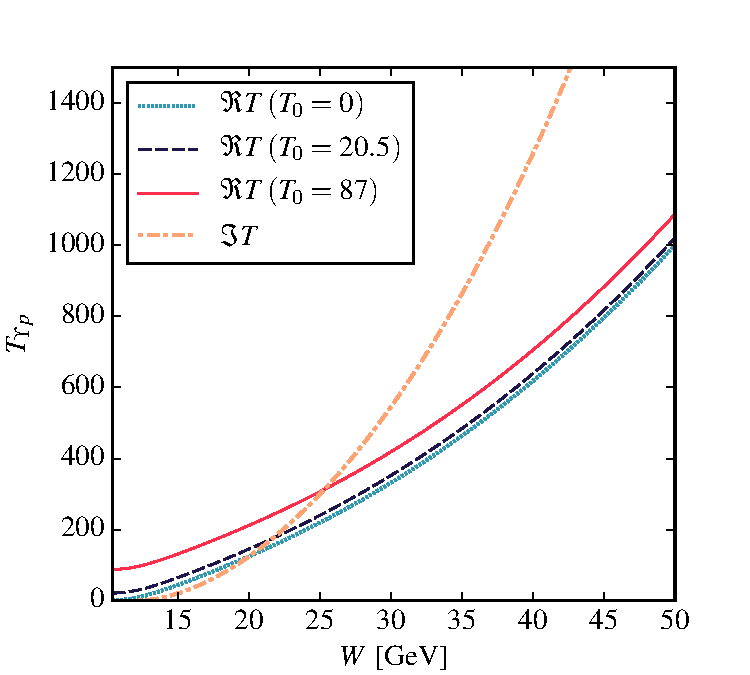
\includegraphics[width=0.49\textwidth]{t_y.pdf}
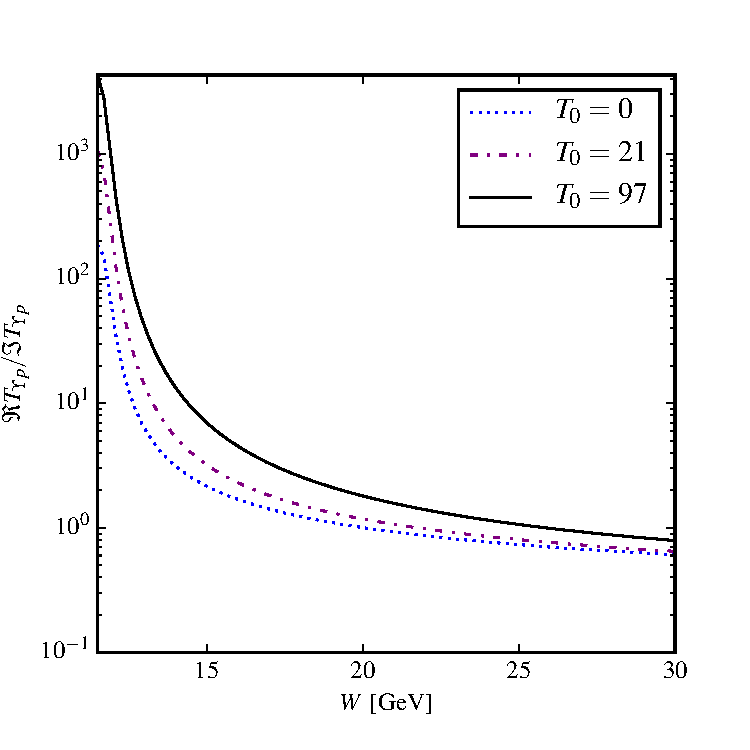
\includegraphics[width=0.49\textwidth]{reimt_y.pdf}
\caption{Left panel:
Imaginary part (dotted curve) and real part of the forward scattering amplitude $T_{\Upsilon p}$ as function of W.
The real part is shown for different values of the subtraction constant as indicated on the figure.
Rigth panel: corresponding ratios of real over imaginary parts plotted starting from inelastic threshold.}
\label{fig:psip_psip}
\end{figure}



We will next simulate $\gamma p \to \Upsilon p$ data in kinematics accessible at a future EIC according to the cross section estimates obtained above, by using the three scenarios for the value of the s-wave scattering length $a_{\Upsilon p}$. 


For the simulations, we consider two beam energies of a future EIC, which are labeled by setting 1 (setting 2), which 
correspond with a collider c.m. energy of 30 GeV (50 GeV) respectively. {\color{red} (CHECK THESE NUMBERS)} 

{\color{red} DISCUSS EIC LUMINOSITY HERE...this would correspond with a one-year running at a luminosity 
${\cal L} = 10^{35}$~cm$^{-2} s^{-1}$ ???   }

For the differential cross section we assume an exponential $t$-dependence according to Eq.~(\ref{eq:bdef}) and normalize its 
value at $t = 0$, given by $A$, to our theoretical estimate for the three choices of the subtraction constant 
$T_{\Upsilon p} (0)$ discussed above. We adjust the $t$-slope $B$ such that it returns the theoretical $\gamma p \to \Upsilon p$ 
total cross section upon integration.  
{\color{red} (CHECK THAT THIS IS WHAT IS DONE IN THE SIMULATION, especially when $-t_{min} \neq 0$)}

In Fig.~\ref{fig:dsigmadt}, we show the simulated results for the $t$-dependence of the $\gamma p \to \Upsilon p$ 
differential cross sections for different values of $W$,  
corresponding with the two EIC beam settings considered.


\begin{figure}[h]
\includegraphics[width=0.49\textwidth]{{dsdt_y_eic1_W_11.5}.pdf}
\includegraphics[width=0.49\textwidth]{{dsdt_y_eic2_W_11.5}.pdf}
\includegraphics[width=0.49\textwidth]{{dsdt_y_eic1_W_21.5}.pdf}
\includegraphics[width=0.49\textwidth]{{dsdt_y_eic2_W_21.5}.pdf}
\includegraphics[width=0.49\textwidth]{{dsdt_y_eic1_W_35.5}.pdf}
\includegraphics[width=0.49\textwidth]{{dsdt_y_eic2_W_35.5}.pdf}
\caption{$t$-dependence of the $\gamma p \to \Upsilon p$ differential cross section 
for different values of the subtraction constant $T_0 \equiv T_{\Upsilon p} (0)$ as indicated on the figure.
The datapoints are simulated based on the theoretical elastic $\Upsilon$ photoproduction cross section, assuming an exponential 
$t$-dependence. The bands represent the uncertainty propagated based on the EIC generated datapoints, 
assuming one-parameter fit of $T_{\Upsilon p}(0)$.}
\label{fig:dsigmadt}
\end{figure}


\begin{figure}
%\includegraphics[width=0.49\textwidth]{dsdt_y.pdf}
%\includegraphics[width=0.49\textwidth]{dsdt_y_close.pdf}
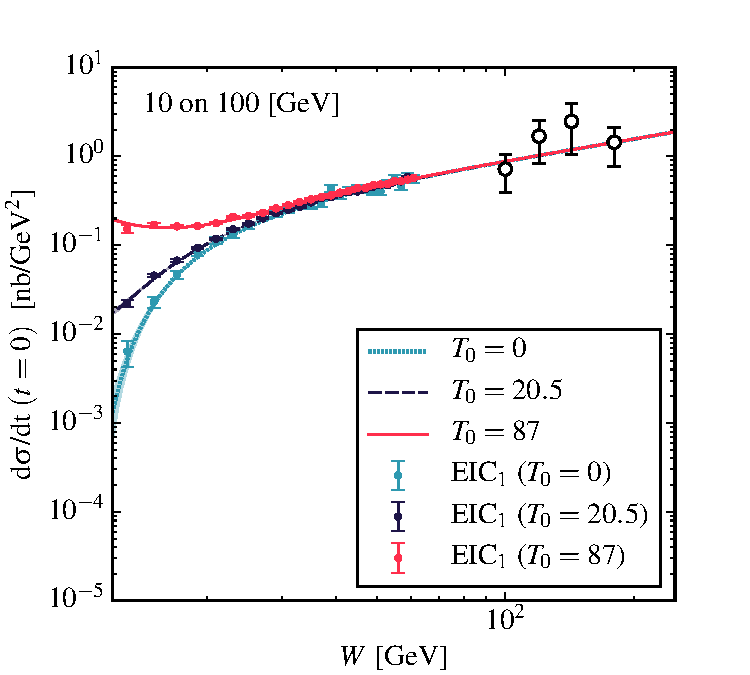
\includegraphics[width=0.49\textwidth]{dsdt_y_eic1.pdf}
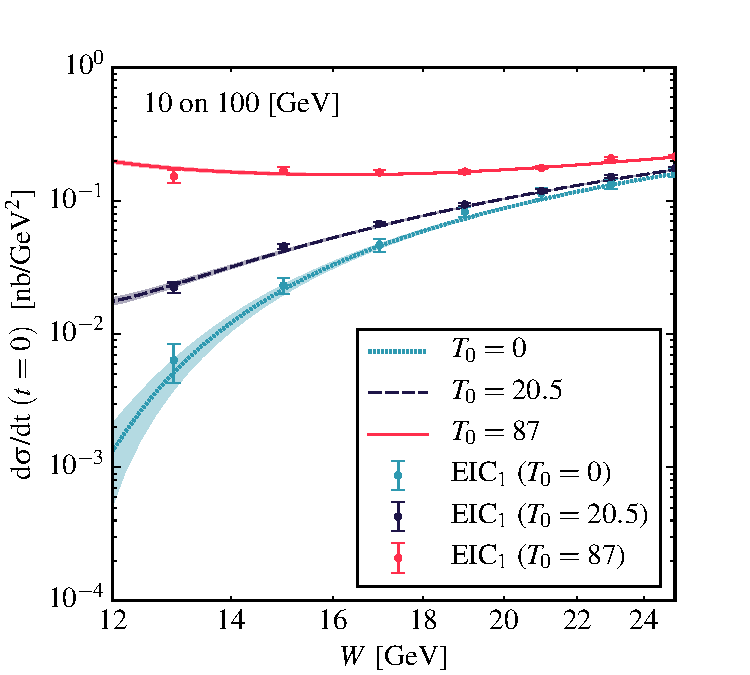
\includegraphics[width=0.49\textwidth]{dsdt_y_close_eic1.pdf}
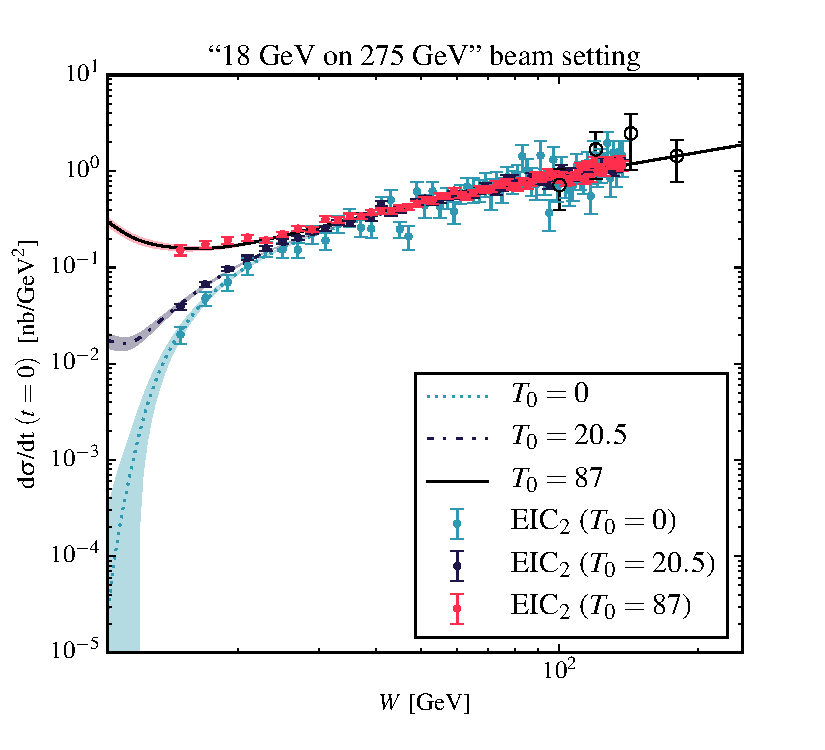
\includegraphics[width=0.49\textwidth]{dsdt_y_eic2.pdf}
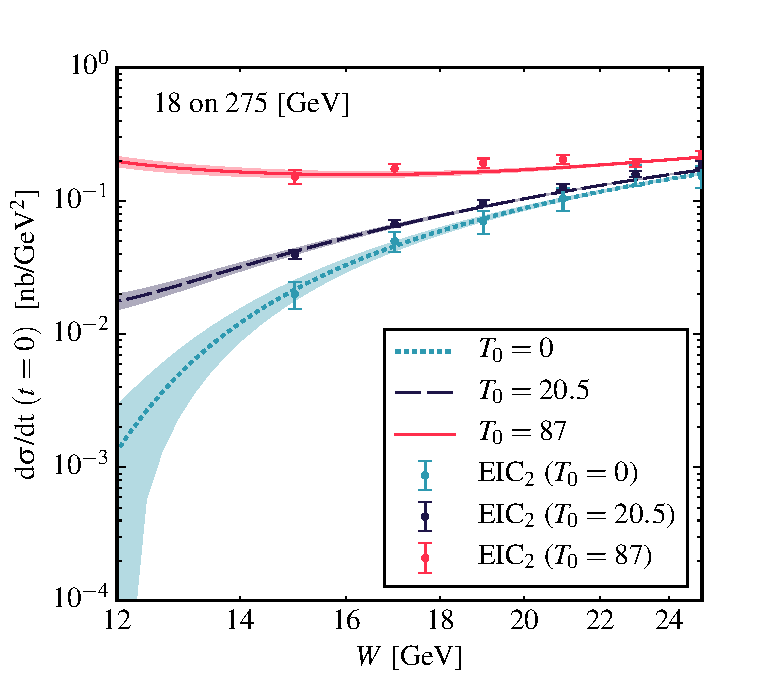
\includegraphics[width=0.49\textwidth]{dsdt_y_close_eic2.pdf}
\caption{W-dependence of the $\gamma p \to \Upsilon p$ differential cross section, extrapolated to the forward direction ($t=0$), 
for different values of the subtraction constant $T_0 \equiv T_{\Upsilon p} (0)$ in the forward $\Upsilon p$ scattering amplitude.
The (black circles) datapoints are obtained from the elastic $\Upsilon$ photoproduction cross section from HERA by using the empirically 
measured slope parameter, using Eq.~(\ref{eq:brel}).
The bands represent the uncertainty propagated based on the EIC generated datapoints,
assuming one-parameter fit of $T_{\Upsilon p}(0)$.}
\label{fig:dsigmadt0}
\end{figure}


\begin{figure}
% \includegraphics[width=0.49\textwidth]{b_slope.pdf}
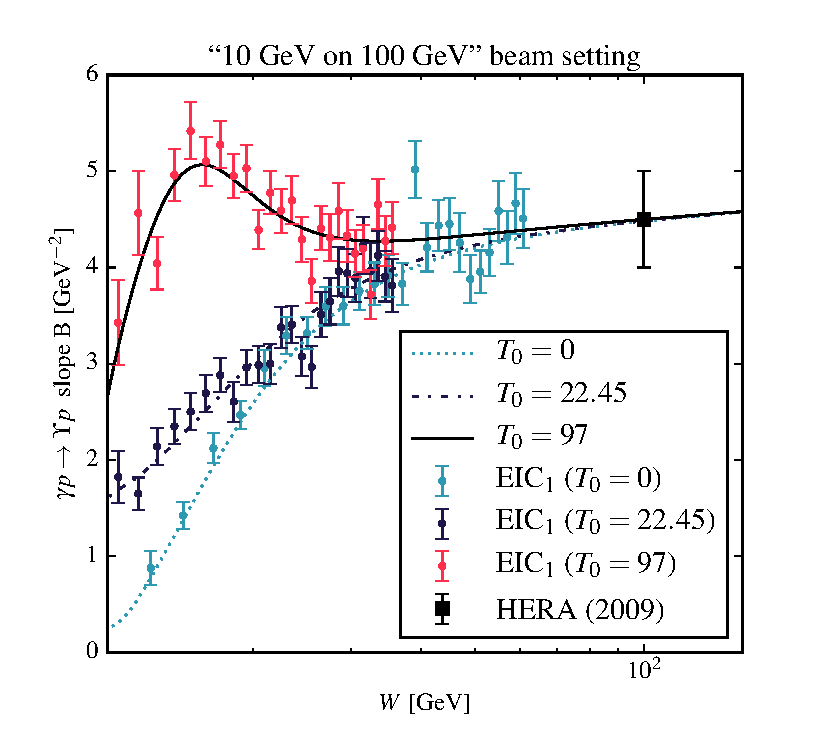
\includegraphics[width=0.49\textwidth]{b_slope_eic1.pdf}
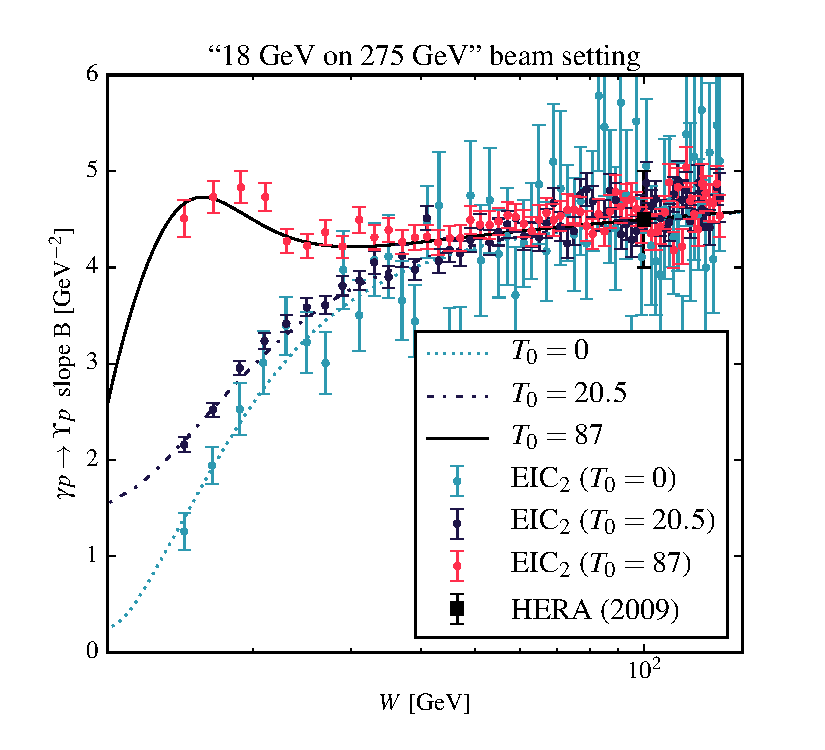
\includegraphics[width=0.49\textwidth]{b_slope_eic2.pdf}
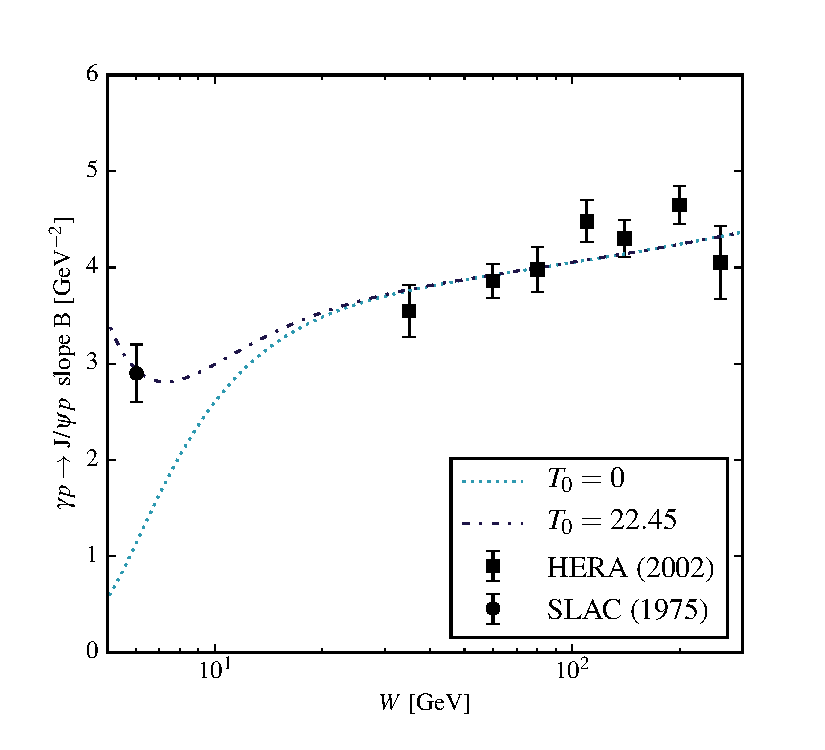
\includegraphics[width=0.49\textwidth]{b_slope_jpsi.pdf}
\caption{
% W-dependence of the left hand side of relation of Eq.~\ref{eq:Crel},
The W-dependence of the B slope parameter introduced in relation \ref{eq:bdef},
for different values of the subtraction constant $T_{\Upsilon p} (0)$ in the forward $\Upsilon p$ (top)
and the forward J/$\psi p $ (bottom) scattering amplitudes.
The value at $W=100$ GeV for the $\Upsilon$ case is $B=4.5\pm0.5$~GeV$^{-2}$~\cite{Chekanov:2009zz}.
The curves shown are obtained by solving Eq.~(\ref{eq:brel}) for $B$.
The $B$ slope data points shown for the J/$\psi$ production are from HERA~\cite{Chekanov:2002xi}.
}
\label{fig:bslope}
\end{figure}

\section{Conclusion}

\section*{Acknowledgements}
The work of OG and MV was supported by the Deutsche Forschungsgemeinschaft (DFG, German Research Foundation),
in part through the Collaborative Research Center [The Low-Energy Frontier of the Standard
Model, Projektnummer 204404729 - SFB 1044], and in part through the Cluster of Excellence
[Precision Physics, Fundamental Interactions, and Structure of Matter] (PRISMA$^+$ EXC
2118/1) within the German Excellence Strategy (Project ID 39083149).



\begin{thebibliography}{99}

%\cite{Gryniuk:2016mpk}
\bibitem{Gryniuk:2016mpk} 
  O.~Gryniuk and M.~Vanderhaeghen,
  %``Accessing the real part of the forward $J/\psi$-p scattering amplitude from $J/\psi$ photoproduction on protons around threshold,''
  Phys.\ Rev.\ D {\bf 94}, no. 7, 074001 (2016)
%  doi:10.1103/PhysRevD.94.074001
%  [arXiv:1608.08205 [hep-ph]].
  %%CITATION = doi:10.1103/PhysRevD.94.074001;%%

\bibitem{Barger:1975ng} 
  V.~D.~Barger and R.~J.~N.~Phillips,
  %``Properties of psi n Scattering,''
  Phys.\ Lett.\ B {\bf 58}, 433 (1975).
%  doi:10.1016/0370-2693(75)90582-1
  %%CITATION = doi:10.1016/0370-2693(75)90582-1;%%
  

\bibitem{Redlich:2000cb} 
  K.~Redlich, H.~Satz and G.~M.~Zinovjev,
  %``Photoproduction constraints on J / psi nucleon interactions,''
  Eur.\ Phys.\ J.\ C {\bf 17}, 461 (2000)
%  doi:10.1007/s100520000488
 % [hep-ph/0003079].
  %%CITATION = doi:10.1007/s100520000488;%%

\bibitem{Kaidalov:1992hd} 
  A.~B.~Kaidalov and P.~E.~Volkovitsky,
  %``Heavy quarkonia interactions with nucleons and nuclei,''
  Phys.\ Rev.\ Lett.\  {\bf 69}, 3155 (1992).
  % doi:10.1103/PhysRevLett.69.3155
  %%CITATION = doi:10.1103/PhysRevLett.69.3155;%%
 
 
%\cite{Adloff:2000vm}
\bibitem{Adloff:2000vm} 
  C.~Adloff {\it et al.} [H1 Collaboration],
  %``Elastic photoproduction of J / psi and Upsilon mesons at HERA,''
  Phys.\ Lett.\ B {\bf 483}, 23 (2000)
  % doi:10.1016/S0370-2693(00)00530-X
%  [hep-ex/0003020].
  %%CITATION = doi:10.1016/S0370-2693(00)00530-X;%%


%\cite{Breitweg:1998ki}
\bibitem{Breitweg:1998ki} 
  J.~Breitweg {\it et al.} [ZEUS Collaboration],
  %``Measurement of elastic Upsilon photoproduction at HERA,''
  Phys.\ Lett.\ B {\bf 437}, 432 (1998)
  % doi:10.1016/S0370-2693(98)01081-8
%  [hep-ex/9807020].
  %%CITATION = doi:10.1016/S0370-2693(98)01081-8;%%
 

%\cite{Chekanov:2009zz}
\bibitem{Chekanov:2009zz} 
  S.~Chekanov {\it et al.} [ZEUS Collaboration],
  %``Exclusive photoproduction of upsilon mesons at HERA,''
  Phys.\ Lett.\ B {\bf 680}, 4 (2009)
  % doi:10.1016/j.physletb.2009.07.066
%  [arXiv:0903.4205 [hep-ex]].
  %%CITATION = doi:10.1016/j.physletb.2009.07.066;%%
 

%\cite{Adloff:1999nr}
\bibitem{Adloff:1999nr} 
  C.~Adloff {\it et al.} [H1 Collaboration],
  %``Measurement of open beauty production at HERA,''
  Phys.\ Lett.\ B {\bf 467}, 156 (1999)
  Erratum: [Phys.\ Lett.\ B {\bf 518}, 331 (2001)]
  % doi:10.1016/S0370-2693(99)01099-0, 10.1016/S0370-2693(01)01035-8
%  [hep-ex/9909029].
  %%CITATION = doi:10.1016/S0370-2693(99)01099-0, 10.1016/S0370-2693(01)01035-8;%%
 

%\cite{Aubert:1981gx}
\bibitem{Aubert:1981gx} 
  J.~J.~Aubert {\it et al.} [European Muon Collaboration],
  %``Observation of Wrong Sign Trimuon Events in 250-{GeV} Muon - Nucleon Interactions,''
  Phys.\ Lett.\  {\bf 106B}, 419 (1981).
  % doi:10.1016/0370-2693(81)90655-9
  %%CITATION = doi:10.1016/0370-2693(81)90655-9;%%
 
\bibitem{Peskin:1979va} 
  M.~E.~Peskin,
  %``Short Distance Analysis for Heavy Quark Systems. 1. Diagrammatics,''
  Nucl.\ Phys.\ B {\bf 156}, 365 (1979).
  % doi:10.1016/0550-3213(79)90199-8
  %%CITATION = doi:10.1016/0550-3213(79)90199-8;%%

 

\bibitem{Chekanov:2002xi} 
  S.~Chekanov {\it et al.} [ZEUS Collaboration],
  %``Exclusive photoproduction of J / psi mesons at HERA,''
  Eur.\ Phys.\ J.\ C {\bf 24}, 345 (2002)
 % doi:10.1007/s10052-002-0953-7
 % [hep-ex/0201043].
  %%CITATION = doi:10.1007/s10052-002-0953-7;%%


\bibitem{Aaij:2015kea}
R.~Aaij \textit{et al.} [LHCb],
%``Measurement of the exclusive Υ production cross-section in pp collisions at $ \sqrt{s}=7 $ TeV and 8 TeV,''
JHEP \textbf{09}, 084 (2015). 
%doi:10.1007/JHEP09(2015)084
%[arXiv:1505.08139 [hep-ex]].


\bibitem{Sirunyan:2018sav}
A.~M.~Sirunyan \textit{et al.} [CMS],
%``Measurement of exclusive $\Upsilon$ photoproduction from protons in pPb collisions at $\sqrt{s_\mathrm{NN}} =$ 5.02 TeV,''
Eur. Phys. J. C \textbf{79}, no.3, 277 (2019). 
%doi:10.1140/epjc/s10052-019-6774-8
%[arXiv:1809.11080 [hep-ex]].

\end{thebibliography}

\end{document}